\let\negmedspace\undefined
\let\negthickspace\undefined
\documentclass[journal]{IEEEtran}
\usepackage[a5paper, margin=10mm, onecolumn]{geometry}
%\usepackage{lmodern} % Ensure lmodern is loaded for pdflatex
\usepackage{tfrupee} % Include tfrupee package

\setlength{\headheight}{1cm} % Set the height of the header box
\setlength{\headsep}{0mm}     % Set the distance between the header box and the top of the text

\usepackage{gvv-book}
\usepackage{gvv}
\usepackage{cite}
\usepackage{amsmath,amssymb,amsfonts,amsthm}
\usepackage{algorithmic}
\usepackage{graphicx}
\usepackage{textcomp}
\usepackage{xcolor}
\usepackage{txfonts}
\usepackage{listings}
\usepackage{enumitem}
\usepackage{mathtools}
\usepackage{gensymb}
\usepackage{comment}
\usepackage[breaklinks=true]{hyperref}
\usepackage{tkz-euclide} 
\usepackage{listings}
% \usepackage{gvv}                                        
\def\inputGnumericTable{}                                 
\usepackage[latin1]{inputenc}                                
\usepackage{color}                                            
\usepackage{array}                                            
\usepackage{longtable}                                       
\usepackage{calc}                                             
\usepackage{multirow}                                         
\usepackage{hhline}                                           
\usepackage{ifthen}                                           
\usepackage{lscape}
\usepackage{multicol}

% Marks the beginning of the document
\begin{document}
\bibliographystyle{IEEEtran}
\vspace{3cm}

\title{10.4.ex.13.1}
\author{EE24BTECH11018 - Durgi Swaraj Sharma}

% \maketitle
% \newpage
% \bigskip
{\let\newpage\relax\maketitle}
\renewcommand{\thefigure}{\theenumi}
\renewcommand{\thetable}{\theenumi}
\setlength{\intextsep}{10pt}
\numberwithin{equation}{enumi}
\numberwithin{figure}{enumi}
\renewcommand{\thetable}{\theenumi}
\textbf{Problem:} Find the roots of the following quadratic equations, if they exist, using the quadratic formula:
\brak{i} $3x^2-5x+2=0$ 
\solution 

The roots can be found in multiple methods. We will solve the problem using the Newton-Raphson method, as it works well for our case due to simplicity.\\ 
\textbf{Newton-Raphson method:}

From a starting value $x_0$, we iterate as following:
\begin{align}
  x_{n+1} = x_n - \frac{f\brak{x_n}}{f^{\prime}\brak{x_n}}
\end{align}
If the roots are real, $x_n$ will converge to a root; but if the roots are complex and the coefficients are real, $x_n$ will converge either to an extrema or grow boundlessly if our inital guess is not complex. \\In our case,
\begin{align}
  f\brak{x} &= 3x^2-5x+2\\
  f^{\prime}\brak{x} &= 6x-5
\end{align}
And the update equation will be
\begin{align}
  x_{n+1} = x_n - \frac{3x^2-5x+2}{6x-5}
\end{align}

Taking starting values of $x$ as $x = 10, -10$, in 9 iterations each, we find the roots to be $0.666667$ and $1.000000$. 

\begin{figure}
  \centering
  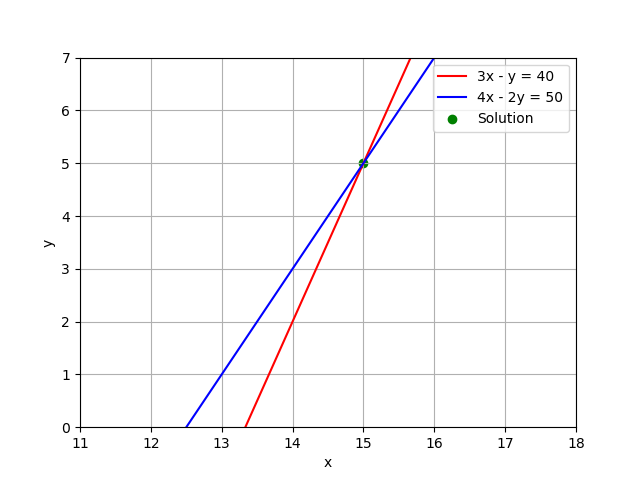
\includegraphics[width=\columnwidth]{/home/gvt1/sdcard/github/EE1003/Assignment4/figs/fig.png}
  \caption{Graphical verification of Newton-Raphson}
\end{figure}

\textbf{Eignenvalue approach:}

By considering the polynomial as the characteristic equation of a matrix, we can find the roots of the polynomial by finding the eigenvalues of the matrix. A companion matrix of a polynomial is a matrix with eigenvalues as the roots of the polynomial. If the polynomial is 
\begin{align}
  P\brak{x}=\sum\limits_{i=0}^n c_ix^{i}\,\text{where }c_n = 1
\end{align}
Then the companion matrix in general, and for our problen is 
\begin{align}
  C &= \begin{bmatrix}
    0&0&\cdots&0&-c_0\\
    1&0&\cdots&0&-c_1\\
    0&1&\cdots&0&-c_2\\
    \vdots&\vdots&\vdots&\ddots&\vdots\\
    0&0&\cdots&1&-c_{n-1}
  \end{bmatrix}\\
  C &= \begin{bmatrix}
    0&\frac{2}{3}\\
    1&\frac{-5}{3}
  \end{bmatrix}
\end{align}

There's multiple algorithms to find the eigenvalues of a matrix. We'll be using the \textbf{QR algorithm} to find the eigenvalues as it is the simplest to understand. Here's a brief explanation of what we'll be doing in the code. 

Let $A$ be a real matrix, let $A_0 = A$. At the $k$th step, we compute the QR dexomposition $A_k = Q_kR_k$, where $Q_k$ is an orthogonal matrix and $R_k$ is an upper triangular matrix. We then form $A_{k+1} = R_kQ_k$. This $A_{k+1}$ is a similar matrix to $A_k$ \brak{\text{same eigenvalues as }A_k} as $A_{k+1} = R_kQ_k = Q^{-1}_kQ_kR_kQ_k = Q^{-1}_kA_kQ_k = Q^T_kA_kQ_k$. Now, running these iterations multiple times, under certain conditions the matrices $A_k$ converge to a triangular matrix called the Schur form of $A$. The eigenvalues of this triangular matrix are listed on the diagonal and the problem is solved. 

The QR decomposition step can be done in many ways too, and we'll be using Householder reflections to perform the decomposition. 

A Householder reflection is a transformation that reflects a vector across a hyperplane. Given a vector $x$, we construct a reflection matrix $H$ such that it zeroes out all but the first entry of $x$. 

The Householder reflection matrix is given by:
\begin{align}
    H = I - 2 \frac{vv^T}{v^T v},
\end{align}
where $v$ is a specially chosen vector such that $Hx$ aligns with a multiple of the standard basis vector $e_1$.

For a given column $a_k$ (the $k$-th column of $A$ starting from row $k$), we define:
\begin{align}
    v = a_k + \text{sign}(a_{k1}) \|a_k\| e_1,
\end{align}
where:
\begin{itemize}
    \item $\|a_k\|$ is the Euclidean norm.
    \item $e_1$ is the standard basis vector with 1 in the first position and zeros elsewhere.
    \item The sign function ensures numerical stability.
\end{itemize}
To transform $A$ into an upper triangular matrix $R$:
\begin{itemize}
    \item Construct $H_1$ to zero out all but the first element of the first column.
    \item Apply $H_1$ to $A$ from the left:
    \begin{align}
        A^{(1)} = H_1 A.
    \end{align}
    \item Construct $H_2$ to zero out all but the first element of the second column (ignoring the first row).
    \item Apply $H_2$ to $A^{(1)}$.
    \item Repeat this process until all subdiagonal elements are zero, yielding an upper triangular matrix $R$.
\end{itemize}

Since each $H_k$ is orthogonal, their product $Q^T = H_m H_{m-1} \dots H_1$ is also orthogonal, so we define:
\begin{align}
    Q = H_1 H_2 \dots H_m.
\end{align}
We now have decomposed $A = QR$, using Householder reflections. Unlike Gram-Schmidt, which can suffer from numerical instability due to loss of orthogonality, Householder reflections maintain high numerical precision. The algorithm has a time complexity of $O(n^3)$, which is comparable to other decomposition methods like Gram-Schmidt but with better numerical stability.  

Repeating this process on $A=RQ$ in multiple iterations, we achieve the Schur form of $A$, with the eigenvalues listed in the diagonal. 

Incase there exist any complex valued eigenvalues, which exist in conjugate pairs, they appear are $2x2$ blocks, which can be resolved to find the complex eigenvalues. 

Now, performing this algorithm on our problem, in $36$ iterations, we find the roots of our equation to be $1.000000$ and $0.666667$. 
\end{document}
